%%%%%%%%%%%%%%%%%%%%%%%%%%%%%%%%%%%%%%%%%
% Last Update: Aaron Hill, August 2014
% 			TTU Atmospheric Science Department
%			aaron.hill@ttu.edu
%%%%%%%%%%%%%%%%%%%%%%%%%%%%%%%%%%%%%%%%%


%%%%%%%%%%%%%%%%%%%%%%%%%%%%%%%%%%%%%%%%%
% This documentclass loads the packages  %
%            setspace                   %
% and                                   %
%           fancyhdr.                   %
% You may have to                        %
% get these if your TeX distribution     %
% doesn't have them.                     %
%%%%%%%%%%%%%%%%%%%%%%%%%%%%%%%%%%%%%%%%%
\documentclass{ttuthes2015}

%%%%%%%%%%%%%%%%%%%%%%%%%%%%%%%%%%%%%%%%%%%%%%
% Include any other add-on  packages you need:%
%%%%%%%%%%%%%%%%%%%%%%%%%%%%%%%%%%%%%%%%%%%%%%
\usepackage{amsmath,amssymb,amsthm,graphicx}
\usepackage{natbib}	       % use for citing notation
\usepackage[nottoc,numbib]{tocbibind}  % include bibliography in table of contents

%%%%%%%%%%%%%%%%%%%%%%%%%%%%%%%%%%
% EDIT  (Running head--  REQUIRED)%
%%%%%%%%%%%%%%%%%%%%%%%%%%%%%%%%%%
\rhead{Texas Tech University, \emph{FirstName MiddleInitial. LastName}, \emph{Month Year}}

%%%%%%%%%%%%%%%%%%%%%%%%%%%%%%%%%%%%%%%%%%%%%%%
% Uncomment if the grad school doesn't like the%
% line under the  running head:                %
%%%%%%%%%%%%%%%%%%%%%%%%%%%%%%%%%%%%%%%%%%%%%%%
\renewcommand{\headrulewidth}{0pt}


%%%%%%%%%%%%%%%%%%%%%%%%%%%%%%%%%%%%%%%%%%%%%%%%%%
%Spacing -- Do you want double or one-and-a-half?%
%%%%%%%%%%%%%%%%%%%%%%%%%%%%%%%%%%%%%%%%%%%%%%%%%%
\doublespacing
%\onehalfspacing

%%%%%%%%%%%%%%%%%%%%%%%%%%%%%%%%%%%%%%%%%%%%%%%%%%%%%%%%%%%%%
%Leave the one you want uncommented.                        %
%In places where single-line-spacing is appropriate         %
%e.g, extended quotations, you can enclose the material     %
%in a singlespacing environment (with \begin{singlespacing} %
% ...  \end{singlespacing}                                  %
%%%%%%%%%%%%%%%%%%%%%%%%%%%%%%%%%%%%%%%%%%%%%%%%%%%%%%%%%%%%%


%%%%%%%%%%%%%%%%%%%%%%%%%%%%%%%%%%%%%%%%%%%%%%%%%%
%Other preamble stuff, e.g., theorem environments%
%or newcommands go here:                         %
% e.g.                                           %
%%%%%%%%%%%%%%%%%%%%%%%%%%%%%%%%%%%%%%%%%%%%%%%%%%
% \newtheorem{theorem}{Theorem}
% \newtheorem{proposition}[theorem]{proposition}
% \newtheorem{question}{Question}
% \newtheorem{conjecture}{Conjecture}
\newcommand{\tab}{\hspace*{2em}}  % tabbing for paragraphs

\bibliographystyle{ametsoc}   % use american meteorological society bibliography style (2014 version)
\bibpunct{(}{)}{;}{a}{}{,}   % set punctuation for citing articles, books, etc. (AMS Style)

\begin{document}



%%%%%%%%%%%%%%%%%%%%%%%%%%%%%%%%%%%%%%%%%%%%%%%%%%%%%%%%
%TITLE PAGE -- Edit the spacing commands after each \\ %
% if necessary                                         %
%%%%%%%%%%%%%%%%%%%%%%%%%%%%%%%%%%%%%%%%%%%%%%%%%%%%%%%%
\begin{titlepage}
\vbox to  \textheight{
\begin{singlespacing}
\begin{center}
"Insert Your Title Here" \\[12pt]  %Edit
by\\[12pt]
FirstName MiddleInitial. LastName, B.S.\\[12pt]   %Edit
A Thesis\\[12pt]   % or Thesis
In\\[12pt]
Atmospheric Science\\[12pt]  % Edit
Submitted to the Graduate Faculty\\
of Texas Tech University in\\
Partial Fulfillment of\\
the Requirements for\\
the Degree of\\[12pt]
MASTERS OF SCIENCES\\[12pt]  %Edit
Approved\\[12pt]
Dr. Committee Chair Name\\ %Edit
Committee Chair\\[12pt]
Dr. Jane Doe\\[12pt] %Edit
Dr. Joe Doe\\[12pt] %Edit
Mark Sheridan\\ %Edit
Dean of the Graduate School\\[12pt]
July, 2020     %Edit
\end{center}
\end{singlespacing}
\vfill}
\end{titlepage}
%%%%%%%%%%%%%%%%%%%
%End of title page%
%%%%%%%%%%%%%%%%%%%

%%%%%%%%%%%%%%%%%%%%%%%%%%%%%%%%%%%%%%%%%%%%%%%%%%%%%%%
%Copyright page -- delete or comment out if not needed%
%usage: \copyrightpage{year of appearance}{Name}      %
%%%%%%%%%%%%%%%%%%%%%%%%%%%%%%%%%%%%%%%%%%%%%%%%%%%%%%%
\copyrightpage{2020}{FirstName MiddleInitial. LastName} %Name should be same as on
%title page
%%%%%%%%%%%%%%%%%%%%%%%%
%\end of copyright page%
%%%%%%%%%%%%%%%%%%%%%%%%

%%%%%%%%%%%%%%%%%%%%%%%
%Start of frontmatter %
%You need this:       %
%%%%%%%%%%%%%%%%%%%%%%%
\frontmatter     % does the numbering and makes new pages


%%%%%%%%%%%%%%%%%%%%%%%%%%%%%
%Acknowledgements           %
%Comment out or delete      %
%if not  wanted             %
%%%%%%%%%%%%%%%%%%%%%%%%%%%%%
\chapter{Acknowledgements}

\tab "insert acknowledgement text here"

%%%%%%%%%%%%%%%%%%%%%%%%%
%End of acknowledgements%
%%%%%%%%%%%%%%%%%%%%%%%%%

%%%%%%%%%%%%%%%%%%%
%Table of Contents%
%%%%%%%%%%%%%%%%%%%
\tableofcontents

%%%%%%%%%%%%%%%%%%%%%%%%%%%%%%%%%%%%%%%%%%%%%%%%%%
%Abstract -- Delete or comment out if not wanted:%
%%%%%%%%%%%%%%%%%%%%%%%%%%%%%%%%%%%%%%%%%%%%%%%%%%
\chapter{Abstract}

\tab "insert abstract text here"

%%%%%%%%%%%%%%%%%
%End of abstract%
%%%%%%%%%%%%%%%%%


%%%%%%%%%%%%%%%%%%%%%%%%%%%%%%%%%%%%%
%List of tables and list of figures %
%Delete or comment out if not needed%
%%%%%%%%%%%%%%%%%%%%%%%%%%%%%%%%%%%%%
\listoftables

\listoffigures
%%%%%%%%%%%%%%%%%%%%%%%%%%%%%%%%%%%%
%End of lists of tables and figures%
%%%%%%%%%%%%%%%%%%%%%%%%%%%%%%%%%%%%

%%%%%%%% OPTIONAL CHAPTER FOR ABBREVIATIONS %%%%%%%%%%%%%
\chapter{List of Abbreviations}
e.g. \\
F - Fahrenheit \\

%%%%%%%%%%%%%%%%%%%%%%%%%%%%%%%%%%%%%%%%%%%%


%%%%%%%%%%%%%%%%%%%%%%%%
%MAIN PART OF  DOCUMENT%
%%%%%%%%%%%%%%%%%%%%%%%%

\mainmatter
\chapter{Introduction}  % how to make a chapter

"Intro text"

\section{Section Title}  % how to make a section

% figure
\tab Make a figure like this
\begin{figure}[!htb]
  \centering
  \noindent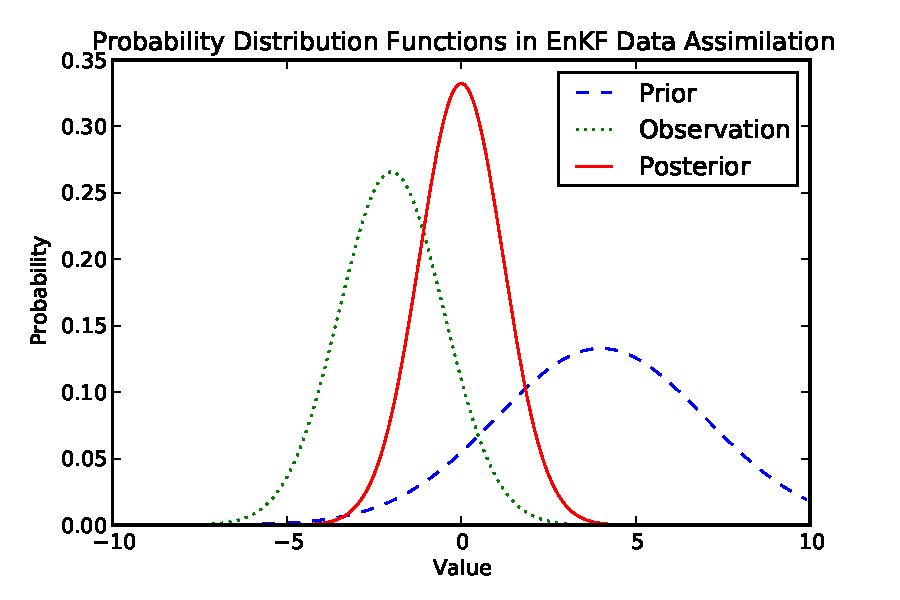
\includegraphics[width=30pc,angle=0]{./example.pdf}\\
  \caption{Example figure and caption}
\label{example}
\end{figure}

\tab Reference a figure: Fig.~$\ref{example}$ \\

% equation
\tab Make an equation like this
\begin{align}\label{J_var}
	\sigma = \frac{1}{M-1} \delta\bf{J} \delta{\mathbf{J}}^T.
\end{align}

\tab Reference an equation: ($\ref{J_var}$) \\
% citing
\tab Ways to Cite (there are more, google them) \\
\citep{Ancell2013} \\
\cite{Ancell2013} \\

\subsection{Subsection Title} % how to make a subsection


%%%%%%%%%%%%%%%%%%%%%%%%%%%%%%%%%%%%%%%%%%%%%%
%Backmatter -- Bibliography, appendices, etc.%
%%%%%%%%%%%%%%%%%%%%%%%%%%%%%%%%%%%%%%%%%%%%%%
\backmatter


%%%%%%%%%%%%%%%%%%%%%%%%%%%%%%%%%%%%%%%%%%%%%%%%%%%%%%%%
%Bibliography:  Use BibTeX if you like. Or enter the items in directly with correct formatting. %
%%%%%%%%%%%%%%%%%%%%%%%%%%%%%%%%%%%%%%%%%%%%%%%%%%%%%%%%

\singlespacing
\bibliography{thesis}

%%%%%%%%%%%%%%%%%%%%%%%%%%%%%%%%%%%%%%%%%%%%%%%%%%%%%%%%
% NOTE: There are small issues with bibliography entry ordering. Edits have to be made in the *.bbl file to align multiple authors correctly
%%%%%%%%%%%%%%%%%%%%%%%%%%%%%%%%%%%%%%%%%%%%%%%%%%%%%%%%


%\begin{thebibliography}{99}   % use when bibtex is not

%%%%%%%%%% EXAMPLE BIB ENTRY TYPED OUT WITHOUT BIBTEX %%%%%%%%%%%%%%
%Ancell, B., and G. J. Hakim, 2007: \emph{Comparing adjoint- and ensemble-sensitivity analysis with applications to observation targeting}. Mon. Wea. Rev., 135, 411--4134.
%\newline\newline
%%%%%%%%%%%%%%%%%%%%%%%%%%%%%%%%%%%%%%%%%%%%%%%%%%%%

%\end{thebibliography}

%%%%%%%%%%%%%%%%%%%%%%%%%%%%%%%%%%%%%%%%%%%%%
%If there's only one appendix, just call it %
%"Appendix".  Otherwise, use "Appendix A",  %
%"Appendix B", etc.                         %
%%%%%%%%%%%%%%%%%%%%%%%%%%%%%%%%%%%%%%%%%%%%%
\chapter{Appendix}

%For example, put your computer code here:

\begin{singlespacing}
\begin{verbatim}
#include <iostream>

using namespace std;

int main(){
   cout << "Hello world!\n";
   return  0;
}
\end{verbatim}
\end{singlespacing}

%\chapter{Appendix B}


\end{document}


 
